\section{左手のポジション}
\subsection{ポジションとは}
ネック上での左手の位置のことを{\bf ポジション}と言います(図\addtocounter{figure}{1} \thefigure)。コントラバスにはフレット\footnote{ギターの指板などに見られる、指で押さえる場所の目印となる直線状の突起}がありませんので、代わりに各ポジションの位置関係を身体感覚として身に付ける必要があります。これ以後の章ではポジションを1つずつ習得し、どの位置を押さえると何の音が出るのかを身体で覚えていきましょう。\\

\begin{flushleft}
\begin{minipage}{280pt}
\ \ \ \ 各ポジションはネックの上端から順に番号が振られています。本書では、ベーシストの間で広く認識されている\cite{simandl}のポジション番号に従います(下表参照)。シマンドルは1の指(人指し指)がA線上でイ短調自然短音階(A-H-C-D-E-F-G-A)の音を取るポジションに整数(I、II、III \(\cdots\) VII)を割り当て、それ以外を「中間ポジション」と名付けています。\\

\begin{small}
\begin{center}
表: 本書で使うポジション略記号\\ \ \\
\begin{tabular}{c|ll}
略記号 & \multicolumn{1}{c}{ポジション名} \cite{simandl} & \multicolumn{1}{c}{特徴}\\
\hline
h.p.   & ハーフ・ポジション       & ネックの上端にある\\
I      & 第Iポジション            & \\
II     & 第IIポジション            & \\
\(\roffset{0.6}{\small [}
\begin{tiny}
\begin{array}{c}
{\rm II}\\
{\rm III}\\
\end{array}
\end{tiny}
\)
 & 第II・第IIIの中間ポジション &\\
III    & 第IIIポジション      & 1と4がフラジオレット\\
\(\roffset{0.6}{\small [}
\begin{tiny}
\begin{array}{c}
{\rm III}\\
{\rm IV}\\
\end{array}
\end{tiny}
\)
& 第III・第IVの中間ポジション & \\
IV     & 第IVポジション            & ネックの根元にある\\
V      & 第Vポジション            & \\
\(\roffset{0.6}{\small [}
\begin{tiny}
\begin{array}{c}
{\rm V}\\
{\rm VI}\\
\end{array}
\end{tiny}
\)
& 第V・第VIの中間ポジション & 4の指はここまで\\
VI     & 第VIポジション            & 3の指がフラジオレット\\
\(\roffset{0.6}{\small [}
\begin{tiny}
\begin{array}{c}
{\rm VI}\\
{\rm VII}\\
\end{array}
\end{tiny}
\)
 & 第VI・第VIIの中間ポジション & \\
VII    & 第VIIポジション            & \\
\end{tabular}
\end{center}
\end{small}

\end{minipage}
\hfill
\begin{minipage}{140pt}
\begin{center}
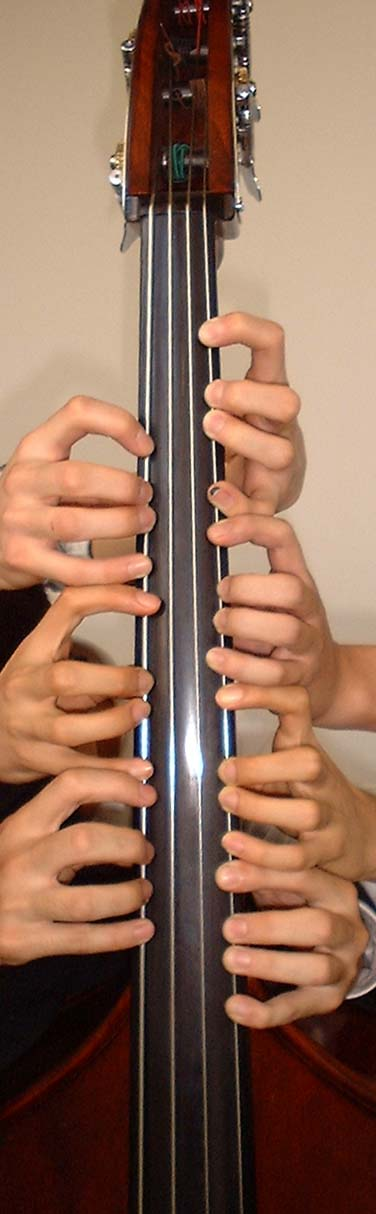
\includegraphics[height=10cm]{../Vol1/Pics/Position/1st-4th.epsi}\\
{\flushleft\small 図\thefigure : 各ポジションの位置関係\\}
\end{center}
\end{minipage}
\end{flushleft}

\subsection{学習の順序}
通常、各ポジションの習得はネックの上端にあるハーフ・ポジションから開始し、徐々にネックの根元の方へと進んで行きます(手の位置が地面に近付くと弾ける音域は上がります)。しかし、ハーフ・ポジションは他のポジションにはない下記のような特徴があるため、
慣れるまではなにかと体力の要るポジションです。

\begin{enumerate}
\item 指の間を大きく広げる必要がある
\item 握力が要る
\item 腕を高い位置に保つ必要がある
\end{enumerate}

どれも慣れの問題なのですが、初心者には体力的なハードルであることは否めず、挫折の原因となりがちです。そこで本書では、比較的楽に握れる第IVポジションからスタートして、ネック上端のハーフ・ポジションへと進む順序で学習します。

%進める学習プログラムを用意しました。

%従来通りハーフ・ポジションから始める学習プログラムも併せて用意しましたので、自分に向いている方を選ぶことが可能です。\\

%ハーフ、第I、第II、第III、第IVの5ポジションの学習が終わったら、それ以降はどちらのコースでも共通の内容になります。
